% BTVN_B8.tex — de TDMXX21, co ban ve khong gian Oxyz (PB12).
% Theo phong cach BTVN_B6.tex; hinh TikZ, khong can tep anh ngoai.
\documentclass[12pt,a4paper]{article}
\usepackage[left=15mm,right=15mm,top=14mm,bottom=18mm,footskip=9mm]{geometry}
\usepackage{iftex}
\ifPDFTeX
  \usepackage[T5]{fontenc}\usepackage[utf8]{inputenc}\usepackage{mathptmx}
\else
  \usepackage{fontspec}
  \IfFontExistsTF{Times New Roman}{\setmainfont{Times New Roman}}{%
    \IfFontExistsTF{Liberation Serif}{\setmainfont{Liberation Serif}}{\setmainfont{Latin Modern Roman}}}
\fi
\usepackage{amsmath,amssymb,fix-cm}
\usepackage{tikz}
\usetikzlibrary{arrows.meta}
\usepackage{tcolorbox,tabularx,fancyhdr,lastpage,needspace}
\definecolor{sectionpurple}{RGB}{155,42,143}
\definecolor{notebackground}{RGB}{229,240,245}
\definecolor{noteborder}{RGB}{255,55,55}
\definecolor{grblue}{RGB}{37,77,194}
\setlength{\parindent}{0pt}
\setlength{\parskip}{0pt}
\setlength{\headheight}{15pt}
\pagestyle{fancy}\fancyhf{}
\renewcommand{\headrulewidth}{0pt}\renewcommand{\footrulewidth}{0.4pt}
\fancyfoot[L]{\fontsize{8.5}{10}\selectfont Biên soạn: \textbf{Nguyễn Anh Dũng}}
\fancyfoot[R]{\fontsize{8.5}{10}\selectfont Trang \thepage/\pageref{LastPage} -- BTVN B8}
\newtcolorbox{notebox}{colback=notebackground,colframe=noteborder,
 boxrule=.65pt,arc=1.5pt,left=5pt,right=5pt,top=2pt,bottom=2pt,
 before skip=0pt,after skip=0pt}
\newcommand{\question}[2][TDM31]{%
  \par\noindent\textbf{\textcolor{sectionpurple}{Câu #2:} \textcolor{noteborder}{[#1]}}\enspace}
\newcommand{\answerlabel}[1]{\textbf{\textcolor{sectionpurple}{#1.}}}
\newcommand{\fourchoices}[4]{%
 \par\nobreak\vspace{1pt}\begin{tabular*}{\linewidth}{@{}l@{\extracolsep{\fill}}lll@{}}
 \answerlabel{A} #1 & \answerlabel{B} #2 & \answerlabel{C} #3 & \answerlabel{D} #4
 \end{tabular*}\par}
\newcommand{\twochoices}[4]{%
 \par\nobreak\vspace{1pt}\begin{tabularx}{\linewidth}{@{}>{\raggedright\arraybackslash}X>{\raggedright\arraybackslash}X@{}}
 \answerlabel{A} #1 & \answerlabel{B} #2 \\[1pt]
 \answerlabel{C} #3 & \answerlabel{D} #4
 \end{tabularx}\par}
\newcommand{\tfbox}[4]{%
\begin{notebox}\renewcommand{\arraystretch}{1.17}\setlength{\tabcolsep}{4pt}
\begin{tabularx}{\linewidth}{|>{\bfseries\color{sectionpurple}}c|>{\raggedright\arraybackslash}X|c|c|}
\hline\multicolumn{2}{|c|}{\textbf{\textcolor{sectionpurple}{Mệnh đề}}}&
\textbf{\textcolor{sectionpurple}{Đ}}&\textbf{\textcolor{sectionpurple}{S}}\\\hline
 a & #1 & $\bigcirc$ & $\bigcirc$ \\ \hline
 b & #2 & $\bigcirc$ & $\bigcirc$ \\ \hline
 c & #3 & $\bigcirc$ & $\bigcirc$ \\ \hline
 d & #4 & $\bigcirc$ & $\bigcirc$ \\ \hline
\end{tabularx}\end{notebox}}
\newcommand{\shortanswer}{%
 \par\nobreak\hfill
\begin{tikzpicture}[baseline=-.7ex]
 \node[draw=noteborder,fill=notebackground,line width=.6pt,rounded corners=1pt,
 minimum width=23mm,minimum height=5mm,inner sep=0pt] {};
 \end{tikzpicture}\par}
\newcommand{\examtitle}[2]{%
 \par\begin{center}\textbf{ĐỀ #1}\\[-1pt]\textbf{#2}\\[-1pt]
 {\fontsize{10.5}{12}\selectfont\itshape Form đề chuẩn bám sát BGD2026 -- Thời gian làm bài \textbf{90 phút}}\end{center}\vspace{-7pt}}
\newcommand{\partone}[1]{\par\textbf{Phần I. Câu trắc nghiệm nhiều phương án lựa chọn.} Thí sinh trả lời từ câu 1 đến câu #1. Mỗi câu chỉ chọn một phương án.\par}
\newcommand{\parttwo}[2]{\par\addvspace{2pt}\textbf{Phần II. Câu trắc nghiệm đúng sai.} Thí sinh trả lời từ câu #1 đến câu #2, trong mỗi ý a), b), c), d) chọn đúng hoặc sai.\par}
\newcommand{\partthree}[2]{\par\addvspace{2pt}\textbf{Phần III. Câu trắc nghiệm trả lời ngắn.} Thí sinh trả lời từ câu #1 đến câu #2.\par}
\newcommand{\finishExam}{\par\vspace{3pt}{\centering\textbf{\textcolor{sectionpurple}{--- Hết ---}}\par}}
% Hinh lap phuong va so do can cau duoc ve bang TikZ theo PDF (TDMXX20).
% Hinh TikZ doc lap, khong can tai tep hinh ben ngoai.
\newcommand{\figbox}[1]{%
\begin{notebox}\centering
\begin{tikzpicture}[x=.43cm,y=.43cm,>=Stealth,every node/.style={font=\fontsize{10}{11}\selectfont}]
 #1
\end{tikzpicture}\end{notebox}}
\newcommand{\axes}[4]{%
 \draw[thin,-{Stealth[length=4pt]}] (#1,0)--(#2,0) node[below] {$x$};
 \draw[thin,-{Stealth[length=4pt]}] (0,#3)--(0,#4) node[right] {$y$};
 \node[below left] at (0,0) {$O$};}
\newcommand{\dotat}[2]{\fill (#1,#2) circle (1.3pt);}
\newcommand{\vguide}[2]{\draw[thin,densely dashed] (#1,0)--(#1,#2);\dotat{#1}{0}\dotat{#1}{#2}}

\newcommand{\cubefig}{%
\begin{notebox}\centering
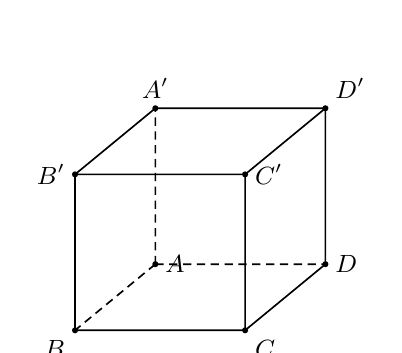
\begin{tikzpicture}[x=.60cm,y=.60cm,line width=.6pt,every node/.style={font=\small}]
 \coordinate (A) at (1.7,1.4); \coordinate (B) at (0,0);
 \coordinate (C) at (3.6,0); \coordinate (D) at (5.3,1.4);
 \coordinate (Ap) at (1.7,4.7); \coordinate (Bp) at (0,3.3);
 \coordinate (Cp) at (3.6,3.3); \coordinate (Dp) at (5.3,4.7);
 \draw[densely dashed] (A)--(B) (A)--(D) (A)--(Ap);
 \draw (B)--(C)--(D)--(Dp)--(Ap)--(Bp)--(B)
       (Bp)--(Cp)--(Dp) (Cp)--(C);
 \foreach \p in {A,B,C,D,Ap,Bp,Cp,Dp}{\fill (\p) circle (1.1pt);}
 \node[right] at (A) {$A$}; \node[below left] at (B) {$B$};
 \node[below right] at (C) {$C$}; \node[right] at (D) {$D$};
 \node[above] at (Ap) {$A'$}; \node[left] at (Bp) {$B'$};
 \node[right] at (Cp) {$C'$}; \node[above right] at (Dp) {$D'$};
\end{tikzpicture}\end{notebox}}
\newcommand{\cranefig}{%
\begin{notebox}\centering
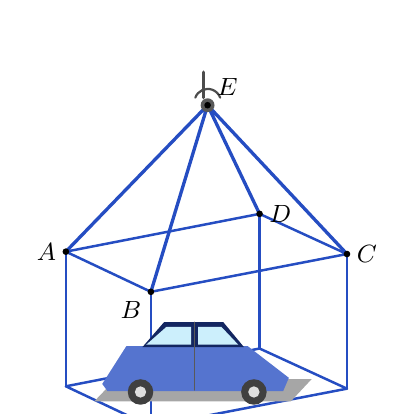
\begin{tikzpicture}[x=.60cm,y=.60cm,line join=round,line cap=round,every node/.style={font=\small}]
 \coordinate (E) at (0,6.15);
 \coordinate (A) at (-3,3.05); \coordinate (B) at (-1.20,2.20);
 \coordinate (C) at (2.95,3.00); \coordinate (D) at (1.10,3.85);
 \coordinate (Ab) at (-3,.20); \coordinate (Bb) at (-1.20,-.65);
 \coordinate (Cb) at (2.95,.15); \coordinate (Db) at (1.10,1.00);
 \draw[line width=1.2pt,grblue] (E)--(A) (E)--(B) (E)--(C) (E)--(D);
 \draw[grblue,line width=.9pt] (A)--(B)--(C)--(D)--cycle;
 \draw[grblue,line width=.9pt] (A)--(Ab) (B)--(Bb) (C)--(Cb) (D)--(Db);
 \draw[grblue,line width=.9pt] (Ab)--(Bb)--(Cb)--(Db)--cycle;
 \draw[very thick,gray!60!black] (-.08,6.85)--(-.08,6.31);
 \fill[gray!70!black] (E) circle (2.5pt);
 \draw[thick,gray!60!black] (-.26,6.31) arc[start angle=160,end angle=20,radius=.28];
 \fill[black!35] (-2.40,-.12)--(1.76,-.12)--(2.20,.35)--(-1.95,.35)--cycle;
 \fill[grblue!78] (-2.23,.25)--(-1.72,1.05)--(.85,1.05)--(1.72,.38)--(1.60,.10)--(-2.12,.10)--cycle;
 \fill[grblue!50!black] (-1.38,1.03)--(-.92,1.56)--(.33,1.56)--(.77,1.03)--cycle;
 \fill[cyan!20] (-1.30,1.08)--(-.87,1.46)--(-.35,1.46)--(-.35,1.08)--cycle;
 \fill[cyan!20] (-.20,1.08)--(-.20,1.46)--(.29,1.46)--(.65,1.08)--cycle;
 \draw[black!65,thin] (-.27,.12)--(-.27,1.56);
 \fill[black!75] (-1.42,.08) circle (.27) (.98,.08) circle (.27);
 \fill[gray!25] (-1.42,.08) circle (.12) (.98,.08) circle (.12);
 \foreach \p/\where in {E/above right,A/left,B/below left,C/right,D/right}
    {\fill (\p) circle (1.2pt);\node[\where] at (\p) {$\p$};}
\end{tikzpicture}\end{notebox}}

\begin{document}
\fontsize{11.5}{14}\selectfont
\examtitle{TDMXX21}{CƠ BẢN VỀ KHÔNG GIAN OXYZ}
\partone{12}

\question[TDM21]{1} Trong không gian $Oxyz$, cho vectơ $\vec{u}=2\vec{i}-3\vec{j}+4\vec{k}$. Tọa độ của vectơ $\vec{u}$ là
\fourchoices{$(2;-3;4)$.}{$(2;0;0)$.}{$(1;-2;4)$.}{$(3;2;4)$.}

\question[TDM21]{2} Trong không gian $Oxyz$, cho vectơ $\vec{u}=3\vec{j}+2\vec{i}-\vec{k}$. Tọa độ của vectơ $\vec{u}$ là
\fourchoices{$(3;2;-1)$.}{$(2;3;0)$.}{$(3;2;0)$.}{$(2;3;-1)$.}

\question[TDM21]{3} Trong không gian $Oxyz$, cho vectơ $\vec{u}=2\vec{i}+3\vec{j}-3\vec{k}$. Tọa độ của vectơ $\vec{u}$ là
\fourchoices{$(2;3;-3)$.}{$(3;4;-1)$.}{$(5;0;-3)$.}{$(2;3;-1)$.}

\question[TDM21]{4} Trong không gian $Oxyz$, cho vectơ $\vec{u}=\vec{i}+2\vec{j}-3\vec{k}$; $\vec{v}=2\vec{i}+\vec{k}$. Tọa độ của vectơ $2\vec{u}+\vec{v}$ tương ứng là
\fourchoices{$(4;4;-5)$.}{$(1;-3;2)$.}{$(2;0;1)$.}{$(2;1;0)$.}

\question[TDM21]{5} Trong không gian với hệ tọa độ $Oxyz$, cho vectơ $\vec{u}=(3;1;-2)$ và vectơ $\vec{v}=(-1;0;3)$. Tọa độ của vectơ $(2\vec{u}+3\vec{v})$ là
\fourchoices{$(2;1;1)$.}{$(3;2;5)$.}{$(3;-2;2)$.}{$(5;1;0)$.}

\question[TDM21]{6} Trong không gian $Oxyz$, cho điểm $A=(-2;3;0)$ và điểm $B=(-1;2;5)$. Tọa độ của vectơ $\overrightarrow{AB}$ tương ứng là
\fourchoices{$(2;-1;0)$.}{$(1;3;-2)$.}{$(1;-1;5)$.}{$(2;-2;3)$.}

\question[TDM31]{7} Trong không gian $Oxyz$, cho hai vectơ $\vec{u}=(m;-3;2)$ và $\vec{v}=(2;n;-4)$, với $m$ và $n$ là hai số thực. Để $\vec{u}$ và $\vec{v}$ cùng phương thì $T=3m+n$ bằng
\fourchoices{$3$.}{$5$.}{$1$.}{$-3$.}

\question[TDM31]{8} Trong không gian $Oxyz$, cho ba điểm $A=(2;3;0)$, $B=(4;0;-2)$, $C=(m;n;3)$. Để $A,B,C$ thẳng hàng thì giá trị của biểu thức $T=7m+2n$ bằng
\fourchoices{$-1$.}{$8$.}{$2$.}{$-3$.}

\question[TDM21]{9} Trong không gian với hệ tọa độ $Oxyz$, cho điểm $A=(3;-2;1)$ và điểm $B=(1;0;-1)$. Độ dài đoạn thẳng $AB$ bằng
\fourchoices{$2\sqrt{3}$.}{$2\sqrt{2}$.}{$3$.}{$2\sqrt{5}$.}

\question[TDM31]{10} Trong không gian $Oxyz$, cho ba điểm có tọa độ là $A=(1;2;3)$, $B=(3;-1;2)$, $C=(-1;2;-2)$. Hãy tìm điểm $D$ sao cho tứ giác $ABCD$ là hình bình hành?
\fourchoices{$(-3;5;-1)$.}{$(3;3;2)$.}{$(2;0;-1)$.}{$(3;1;4)$.}

\question[TDM31]{11} Trong không gian với hệ tọa độ $Oxyz$, cho $4$ điểm có tọa độ là $A=(2;1;0)$, $B=(0;-1;2)$, $C=(2;-1;-1)$, $D=(3;3;1)$. Giá trị \textbf{cosin} góc tạo bởi hai đường thẳng $AB$ và $CD$ bằng
\fourchoices{$\dfrac{1}{\sqrt7}$.}{$-\dfrac{1}{\sqrt7}$.}{$\sqrt{\dfrac67}$.}{$\dfrac{\sqrt7}{3}$.}

\question[TDM31]{12} Trong không gian với hệ tọa độ $Oxyz$, cho hai vectơ $\vec{u}=(3;m;-1)$ và $\vec{v}=(m-1;-2;2)$ vuông góc với nhau. Giá trị của $m$ bằng
\fourchoices{$1$.}{$5$.}{$-2$.}{$3$.}

\parttwo{13}{16}
\question[TDM21]{13} Trong không gian $Oxyz$, cho điểm $M(1;3;4)$. Mệnh đề nào sau đây là \textbf{đúng hay sai}?
\tfbox{Hình chiếu của điểm $M$ trên mặt phẳng $Oxy$ là $M_1(1;3;0)$.}
{Hình chiếu của điểm $M$ trên mặt phẳng $Oyz$ là $M_2(1;0;4)$.}
{Hình chiếu của điểm $M$ trên trục $Oy$ là $M_3(0;3;0)$.}
{Độ dài của vectơ $\overrightarrow{OM}$ là $\sqrt{26}$.}

\question[TDM31]{14} Trong không gian $Oxyz$, cho hai điểm $A(1;-2;5)$ và $B(3;0;1)$. Mệnh đề nào sau đây là \textbf{đúng hay sai}?
\tfbox{Trung điểm của đoạn $AB$ có tọa độ là $(2;-1;3)$.}
{Trọng tâm của tam giác $OAB$ có tọa độ là $(1;1;2)$.}
{Điểm $M$ thỏa mãn $\overrightarrow{MA}-2\overrightarrow{MB}=\vec{0}$ có tọa độ là $(5;2;-3)$.}
{Điểm $N$ thỏa mãn $2\overrightarrow{NO}+3\overrightarrow{NA}-4\overrightarrow{NB}=\vec{0}$ có tọa độ là $(-2;-2;4)$.}

\question[TDM31]{15} Trong không gian $Oxyz$, cho ba điểm $A(1;0;2)$, $B(0;2;3)$, $C(2;-1;0)$. Mệnh đề nào sau đây là \textbf{đúng hay sai}?
\tfbox{$\sin(\overrightarrow{AB},\overrightarrow{AC})=\dfrac{\sqrt{11}}6$.}
{Diện tích tam giác $ABC$ bằng $\dfrac{\sqrt{11}}2$.}
{Bán kính đường tròn ngoại tiếp tam giác $ABC$ bằng $3\sqrt{2}$.}
{Bán kính đường tròn nội tiếp $\triangle ABC$ bằng $0{,}35$. (Làm tròn kết quả đến hàng phần trăm)}

\question[TDM32]{16} Trong không gian $Oxyz$, cho hai vectơ $\vec{a}$ và $\vec{b}$. Mệnh đề nào sau đây là \textbf{đúng hay sai}?
\tfbox{$\vec{a}\cdot\vec{b}\leq |\vec{a}|\cdot|\vec{b}|$.}
{$\vec{a}\cdot\vec{b}\geq-\dfrac12|\vec{a}|\cdot|\vec{b}|$.}
{$|\vec{a}|+|\vec{b}|\geq|\vec{a}+\vec{b}|$.}
{Nếu $\vec{a}=(x;y)$, $\vec{b}=(a;b)$ thì $|\vec{a}|+|\vec{b}|\geq\sqrt{(x-a)^2+(y-b)^2}$.}

\partthree{17}{22}
\question[TDM31]{17} Trong không gian $Oxyz$, cho ba vectơ $\vec{a}=(2;1;0)$, $\vec{b}=(3;-2;1)$, $\vec{c}=(0;2;4)$. Hãy tính giá trị của biểu thức $T=(\vec{a}+2\vec{b})\cdot\vec{c}$ (làm tròn kết quả đến hàng đơn vị)?
\shortanswer

\question[TDM32]{18} Trong không gian $Oxyz$, cho hai điểm $A(1;-3;4)$ và $B(3;1;2)$. Gọi $C,D$ là hai điểm lần lượt nằm trên trục tọa độ $Ox$ và mặt phẳng $(Oyz)$ để tứ giác $ABCD$ là hình bình hành. Hãy xác định hoành độ của điểm $C$?
\shortanswer

\question[TDM32]{19} Trong không gian $Oxyz$, cho điểm $A=(3;1;2)$ và ba điểm $B,C,D$ lần lượt nằm trên ba trục tọa độ $Ox,Oy,Oz$. Để tứ giác $ABCD$ là hình bình hành thì hoành độ của điểm $B$ là
\shortanswer

\question[TDM32]{20} Trong không gian $Oxyz$, cho bốn điểm $A(1;0;0)$, $B(4;0;0)$, $C,D$ theo thứ tự tạo thành một hình vuông. Biết hai điểm $C,D$ nằm trên mặt phẳng $(Oxy)$ và có tung độ dương. Hãy tính khoảng cách $OC$ (làm tròn kết quả đến hàng đơn vị)?
\shortanswer

\question[TDM32]{21} Trong không gian $Oxyz$, cho bốn điểm tạo thành một tứ giác lồi $A(0;0;4)$, $B(2;1;0)$, $C(4;-1;2)$, $D(1;-2;7)$. Diện tích của tứ giác lồi này có giá trị bằng bao nhiêu (làm tròn kết quả đến hàng phần mười)?
\shortanswer

\question[TDM32]{22} Trong không gian $Oxyz$, cho bốn điểm $A(0;1;0)$, $B(0;5;0)$, $C$, $D(2;-1;1)$ theo thứ tự tạo thành một tứ giác lồi nội tiếp một đường tròn. Khi $AC$ lớn nhất hãy tính độ dài cạnh $BC$ (làm tròn kết quả đến hàng đơn vị)?
\shortanswer
\finishExam

% Nguon: DE TDMXX21_DTL_CO BAN VE KHONG GIAN OXYZ_2026_PB12.pdf (3 trang).
% Ban LaTeX: BTVN_B8.tex; giu phong cach va bo cuc BTVN_B7.tex.
\end{document}
